\documentclass[12pt,a4paper]{article}
\usepackage[polish]{babel}
\usepackage[T1]{fontenc}
\usepackage[utf8x]{inputenc}
\usepackage{hyperref}
\usepackage{url}
\usepackage{graphicx}
\usepackage{float}

\addtolength{\hoffset}{-1.5cm}
\addtolength{\marginparwidth}{-1.5cm}
\addtolength{\textwidth}{3cm}
\addtolength{\voffset}{-1cm}
\addtolength{\textheight}{2.5cm}
\setlength{\topmargin}{0cm}
\setlength{\headheight}{0cm}

\begin{document}

\title{Bazy Danych\\Projekt Karta Pacjenta}
\date{\today}

\maketitle

\tableofcontents
\clearpage

% zad 1
\section{Autorzy}
   \large
{
%\textbf{Krzysztof Czarnecki}  - implementacja niewidocznej dla użytkownika części programu, która posiada dostęp do wymaganych zasobów (ang. \textit{backend}) \\
%\textbf{Błażej Czekała} - implementacja testów obciążeniowych, z użyciem wielowątkowości\\
%\textbf{Patryk Wenz} - implementacja wyglądu i zachowania strony (ang. \textit{frontend})\\
%\textbf{Hubert Braun} - implementacja bazy danych i jej obsługi
} 
\section{Opis projektu ,,Karta Pacjenta''}
Projekt ,,Karta Pacjenta'' zakładał stworzenie aplikacji umożliwiającej przechowywanie danych pacjentów w serwisie bazodanowym.
Aplikacja przechowuje informacje dotyczące chorób przebytych przez pacjenta, wystawionych przez lekarza recept.
Umożliwia bezpieczne przechowywanie danych wrażliwych, takich jak pesel, numer telefonu itd.
Umożliwia także prezentację tych danych oraz ich eksport (także w postaci anonimowej - bez danych osobowych -
posiadających tylko informację o przebytej chorobie, nie o pacjencie).

Aplikacja powstała przy użyciu języków: Java (ang. \textit{backend}) oraz Angular (TypeScript) (ang. \textit{frontend}).
Serwis postawiony jest na darmowej domenie dostępnej pod \href{http://trunk-kartapacjenta.herokuapp.com/}{tym linkiem}.
Gorąco zachęcamy do zapoznania się z działaniem aplikacji.

Dzięki serwisowi \href{https://heroku.com/} {Heroku} możliwe było darmowe opublikowanie witryny\\ w internecie.
Nawet w darmowej wersji serwis ten zapewnia usługi związane z CI (ang. \textit{Continuous Integration}).
Efektem tego, jest fakt, że po każdej aktualizacji zdalnego repozytorium \textit{Git} serwis automatycznie przebudowuje się.

\subsection{Przedstawienie aplikacji}

% login page
\begin{figure}[H]
\centering
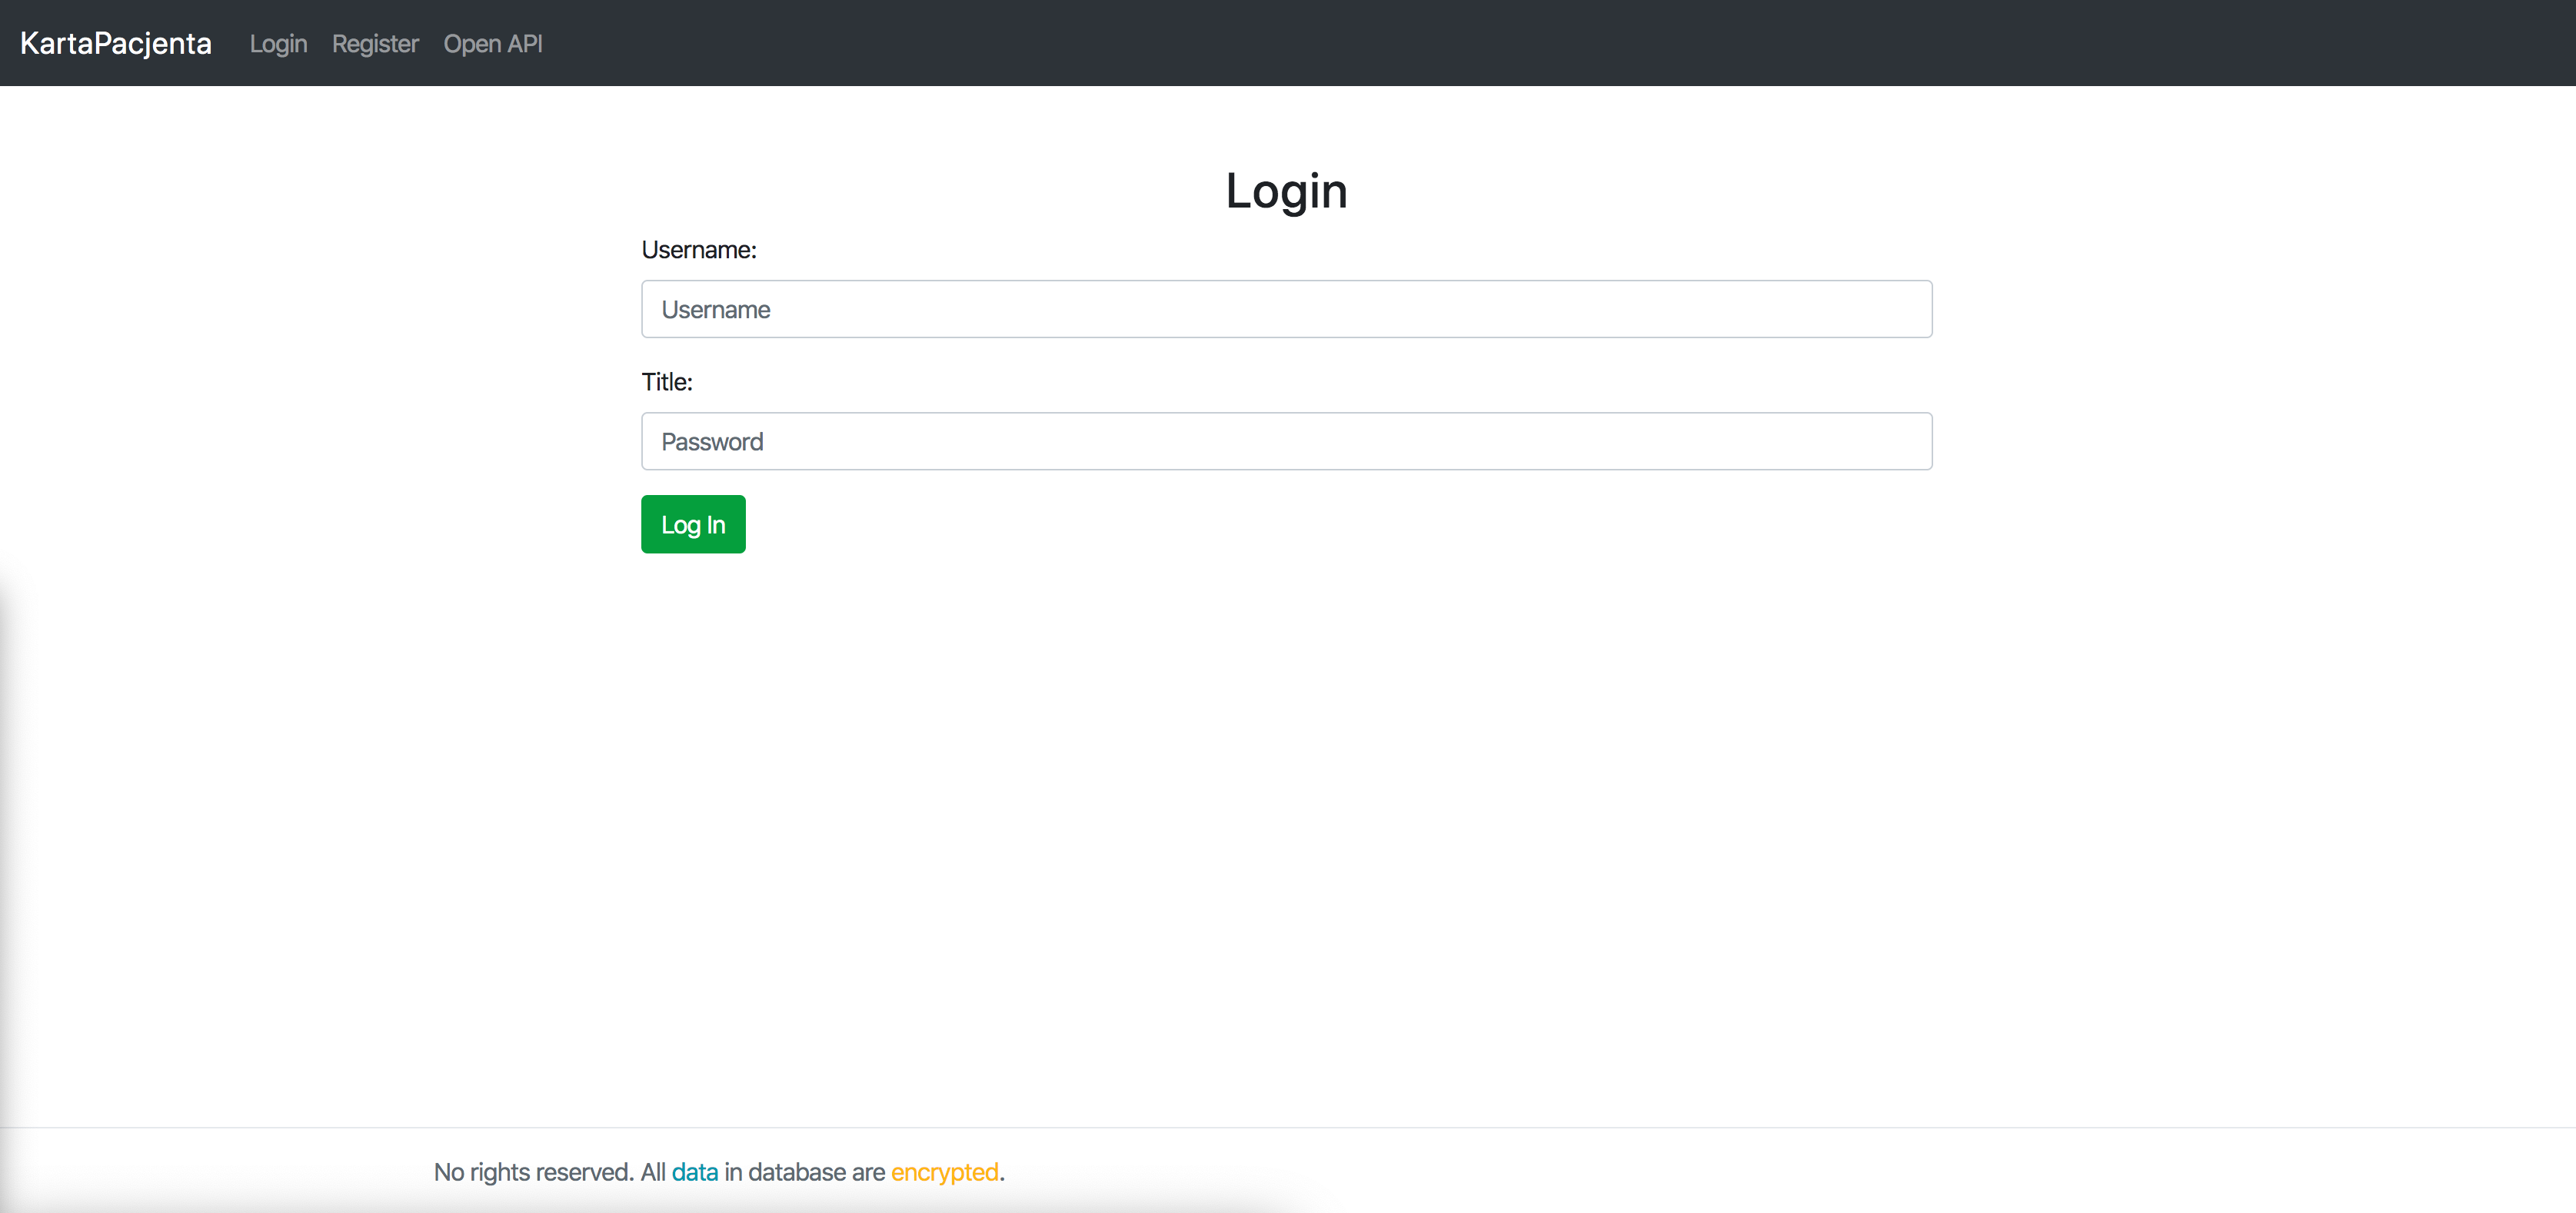
\includegraphics[width=15cm]{pictures/service/01_login}
\caption{Ekran logowania.}
\end{figure}

% admin panel
\begin{figure}[H]
\centering
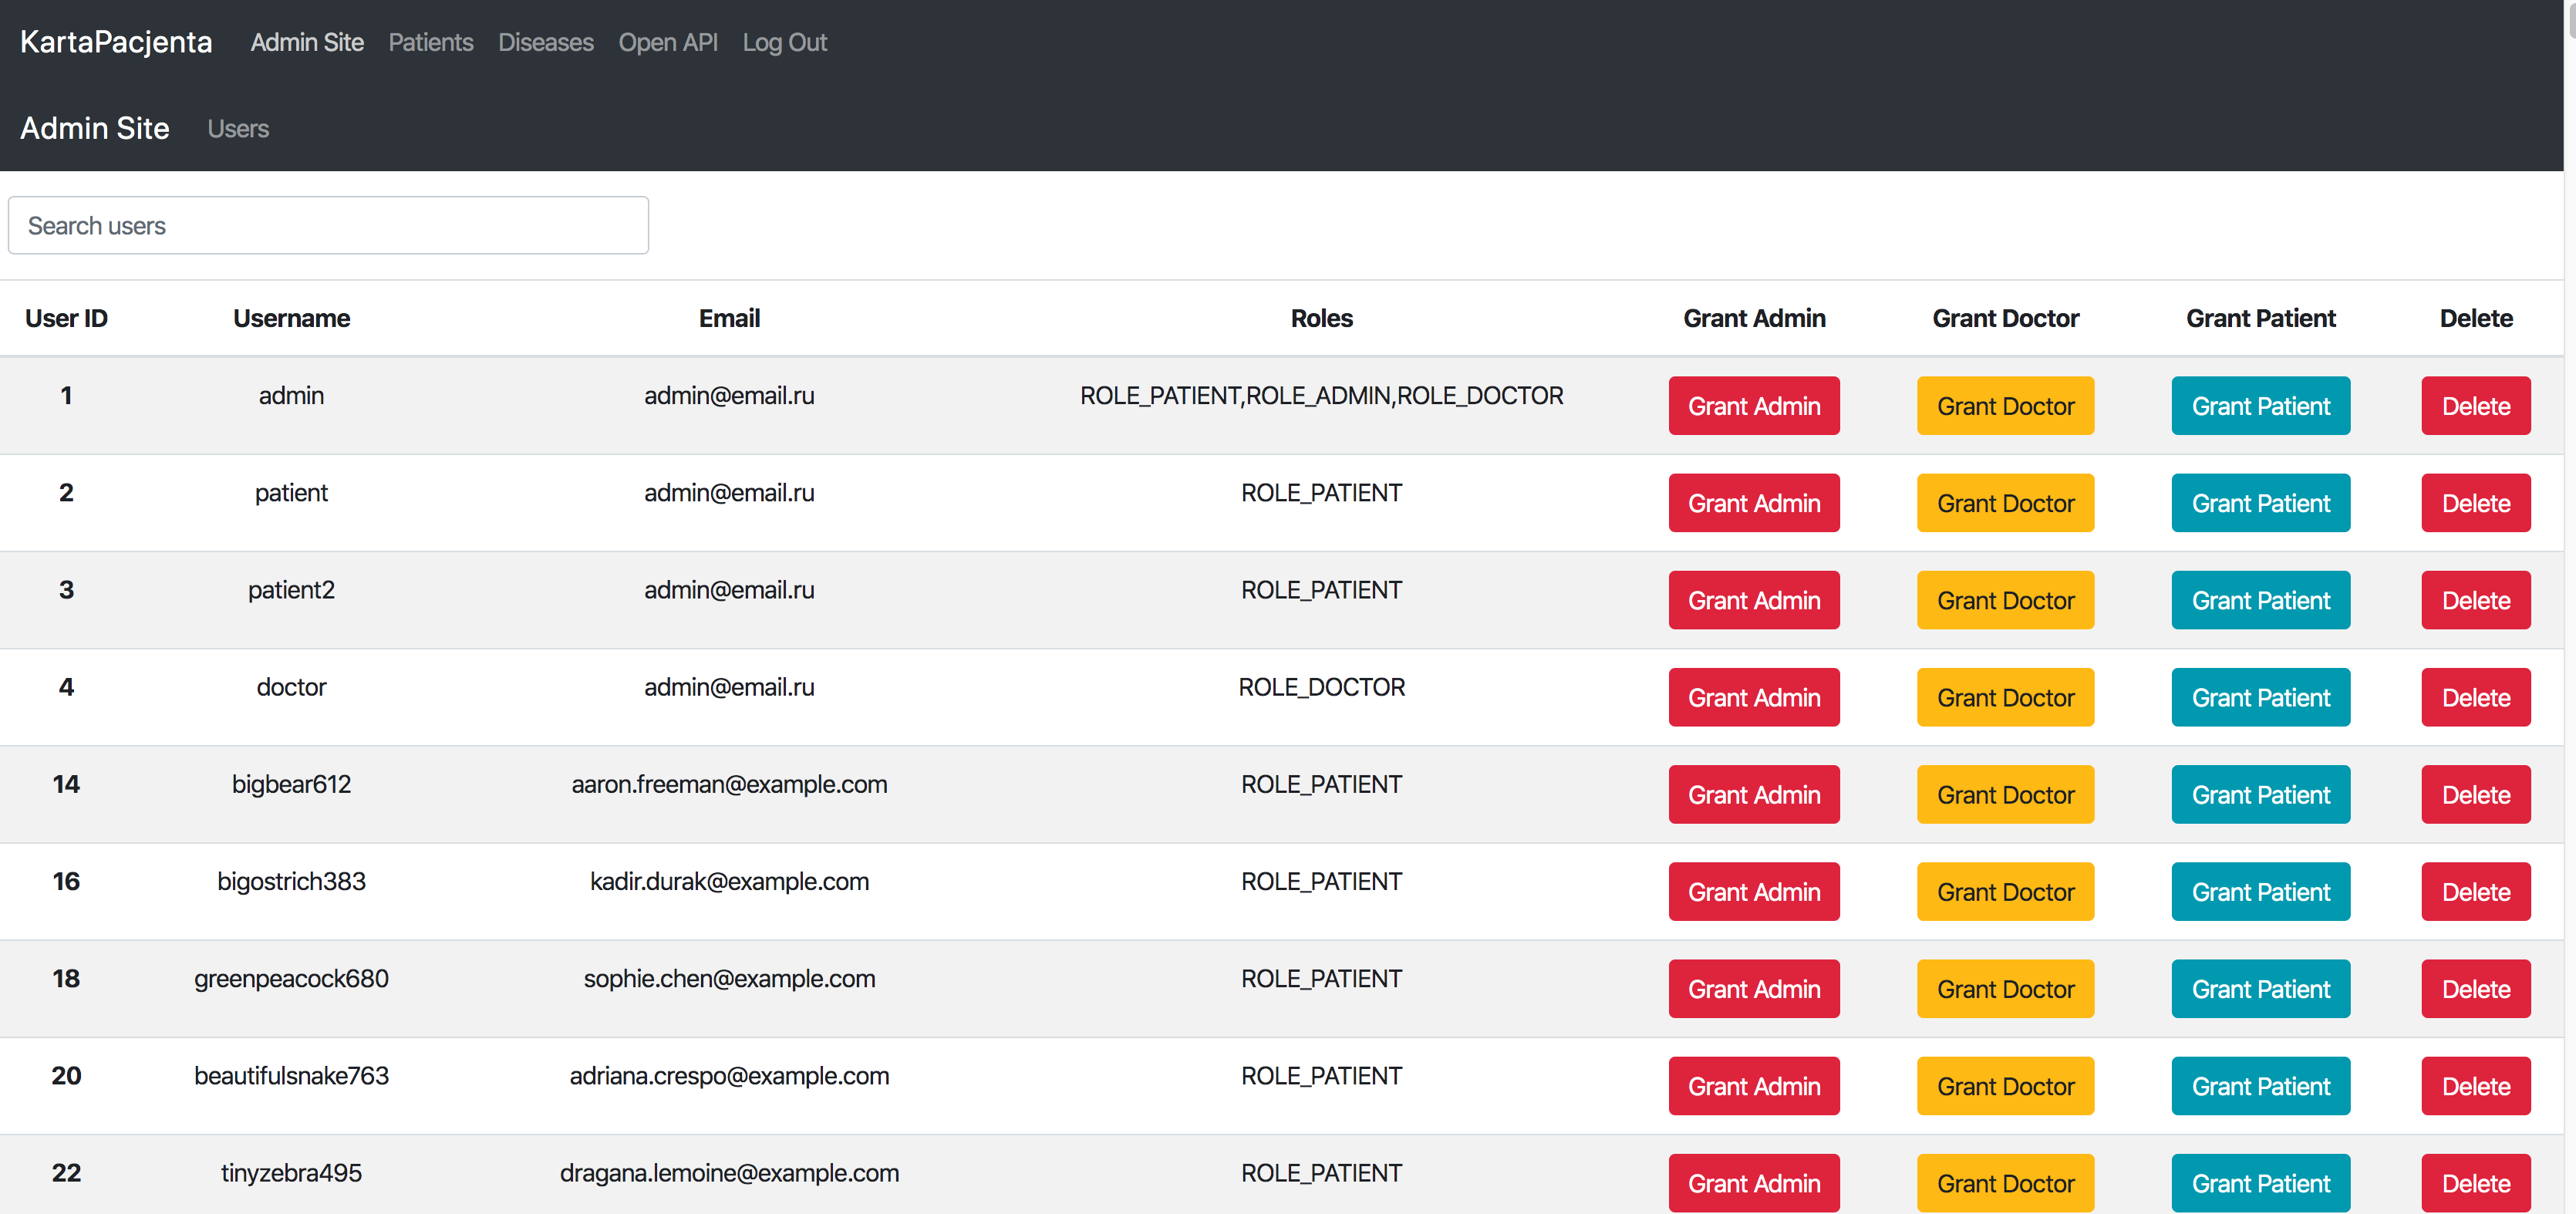
\includegraphics[width=15cm]{pictures/service/02-admin_panel}
\caption{Panel administratora, umożliwiający nadawanie praw, oraz usuwanie użytkowników.}
\end{figure}

% choroby
\begin{figure}[H]
\centering
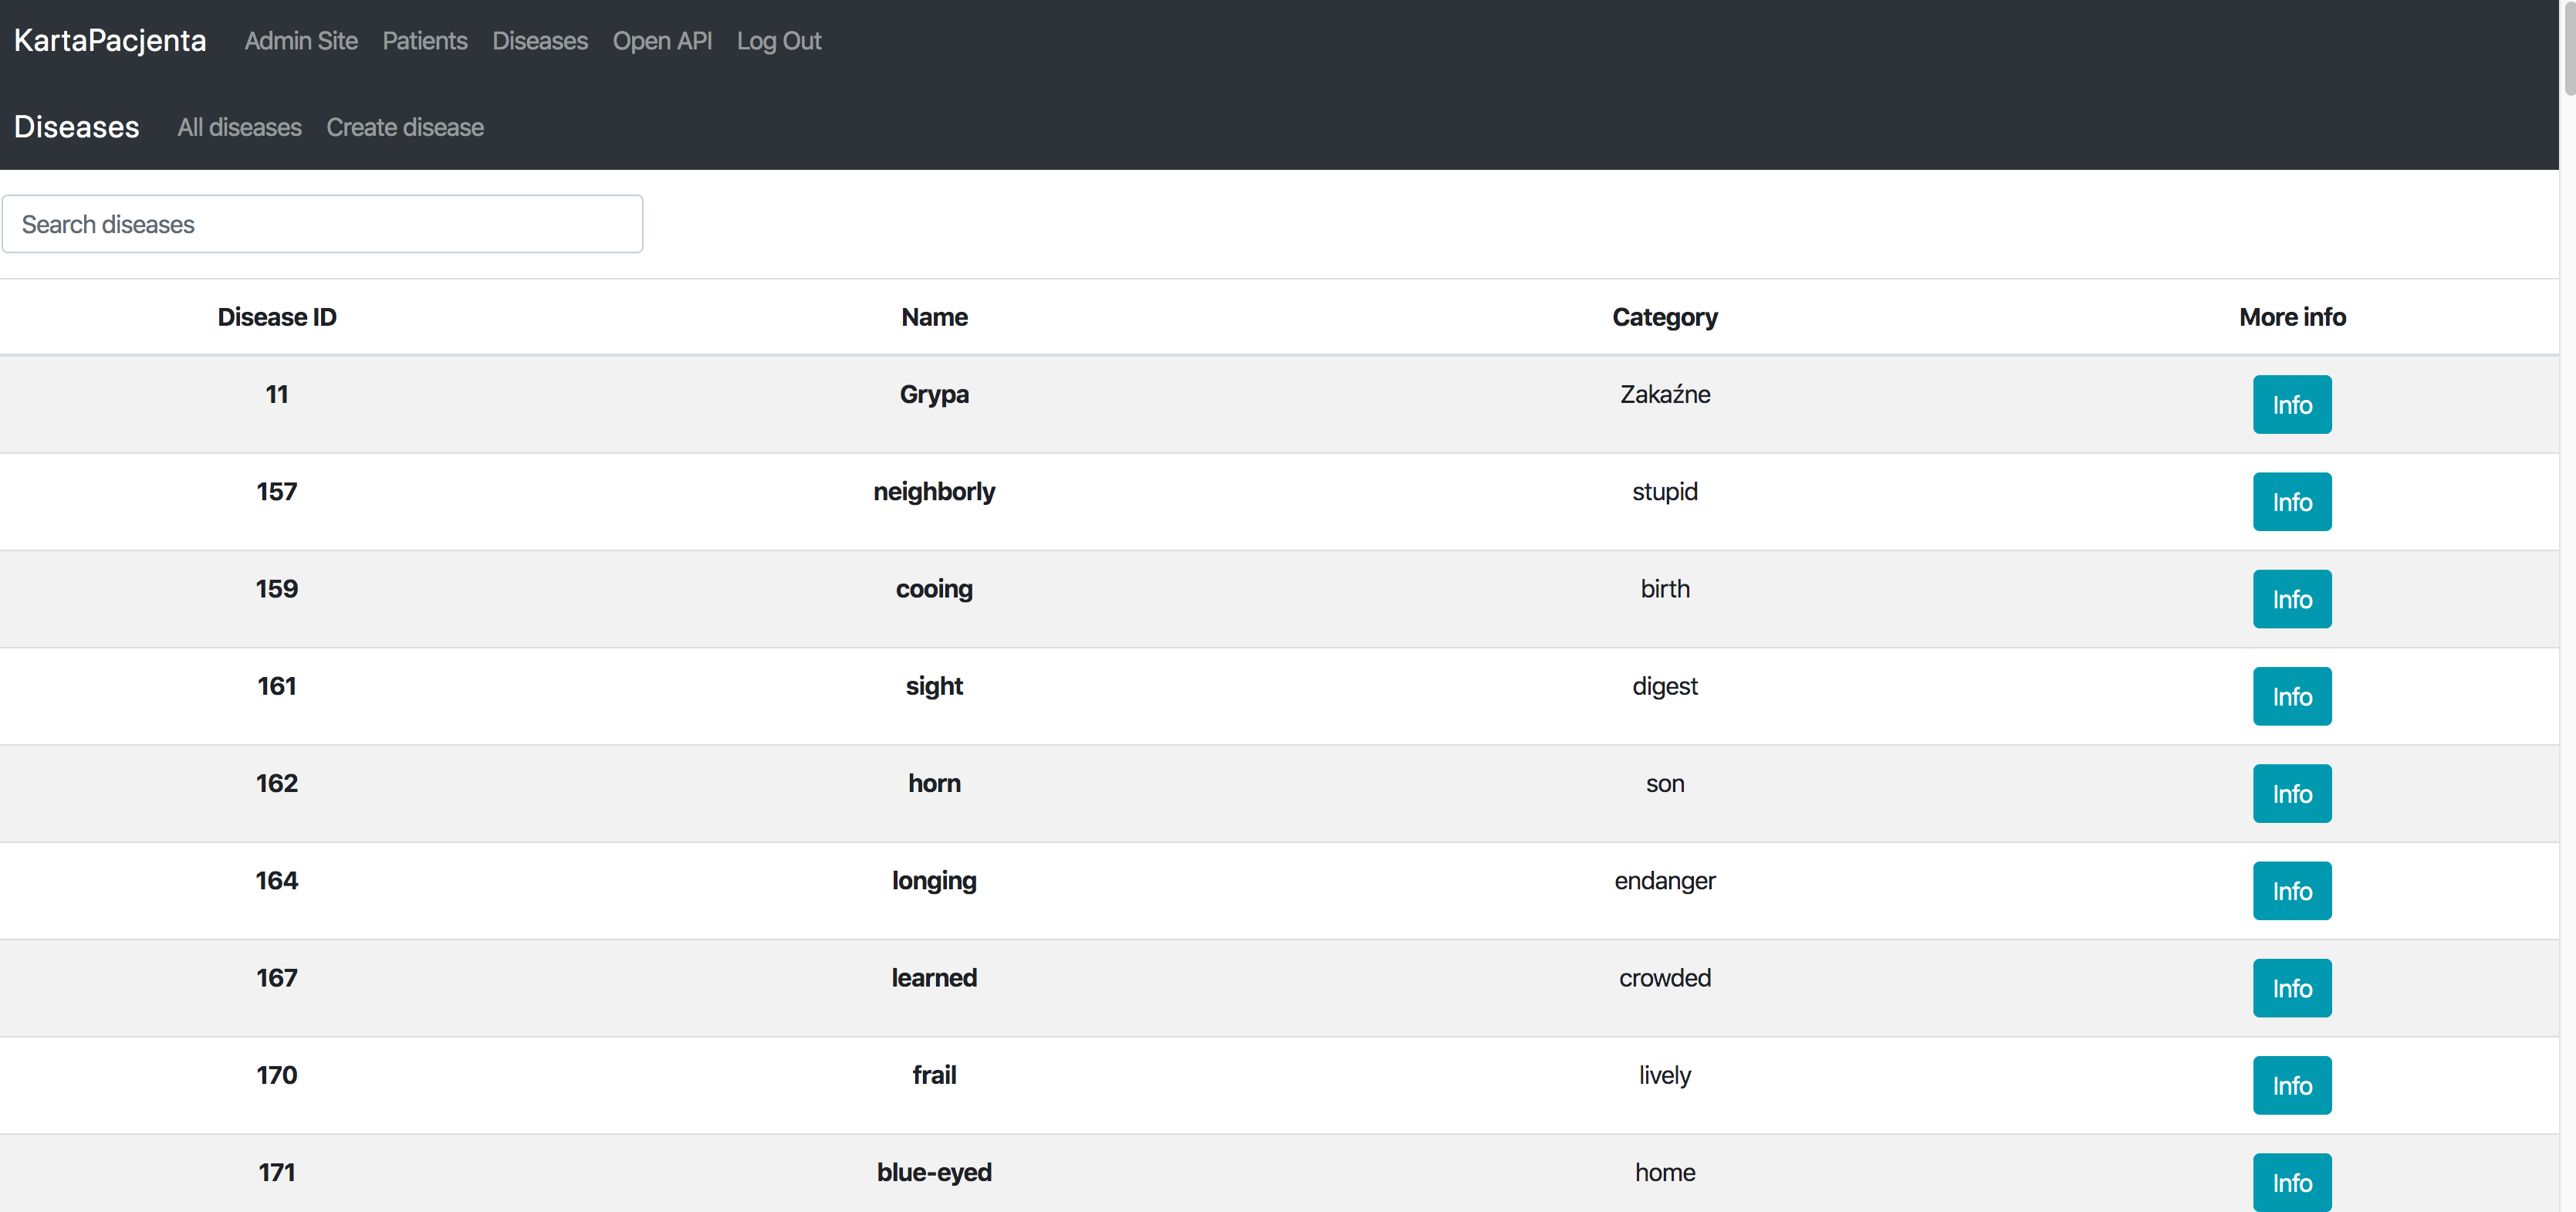
\includegraphics[width=15cm]{pictures/service/04-choroby}
\caption{Zakładka zawierająca wypisane wszystkie zapisane w systemie choroby.
Obok widoczna zakładka umożliwiająca dodanie nowej choroby. Przycisk \textit{,,info''} w tabeli \textit{,,More info''}
umożliwia zapoznanie się z dostępnymi informacjami dotyczącymi danej choroby.}
\end{figure}

% patients
\begin{figure}[H]
\centering
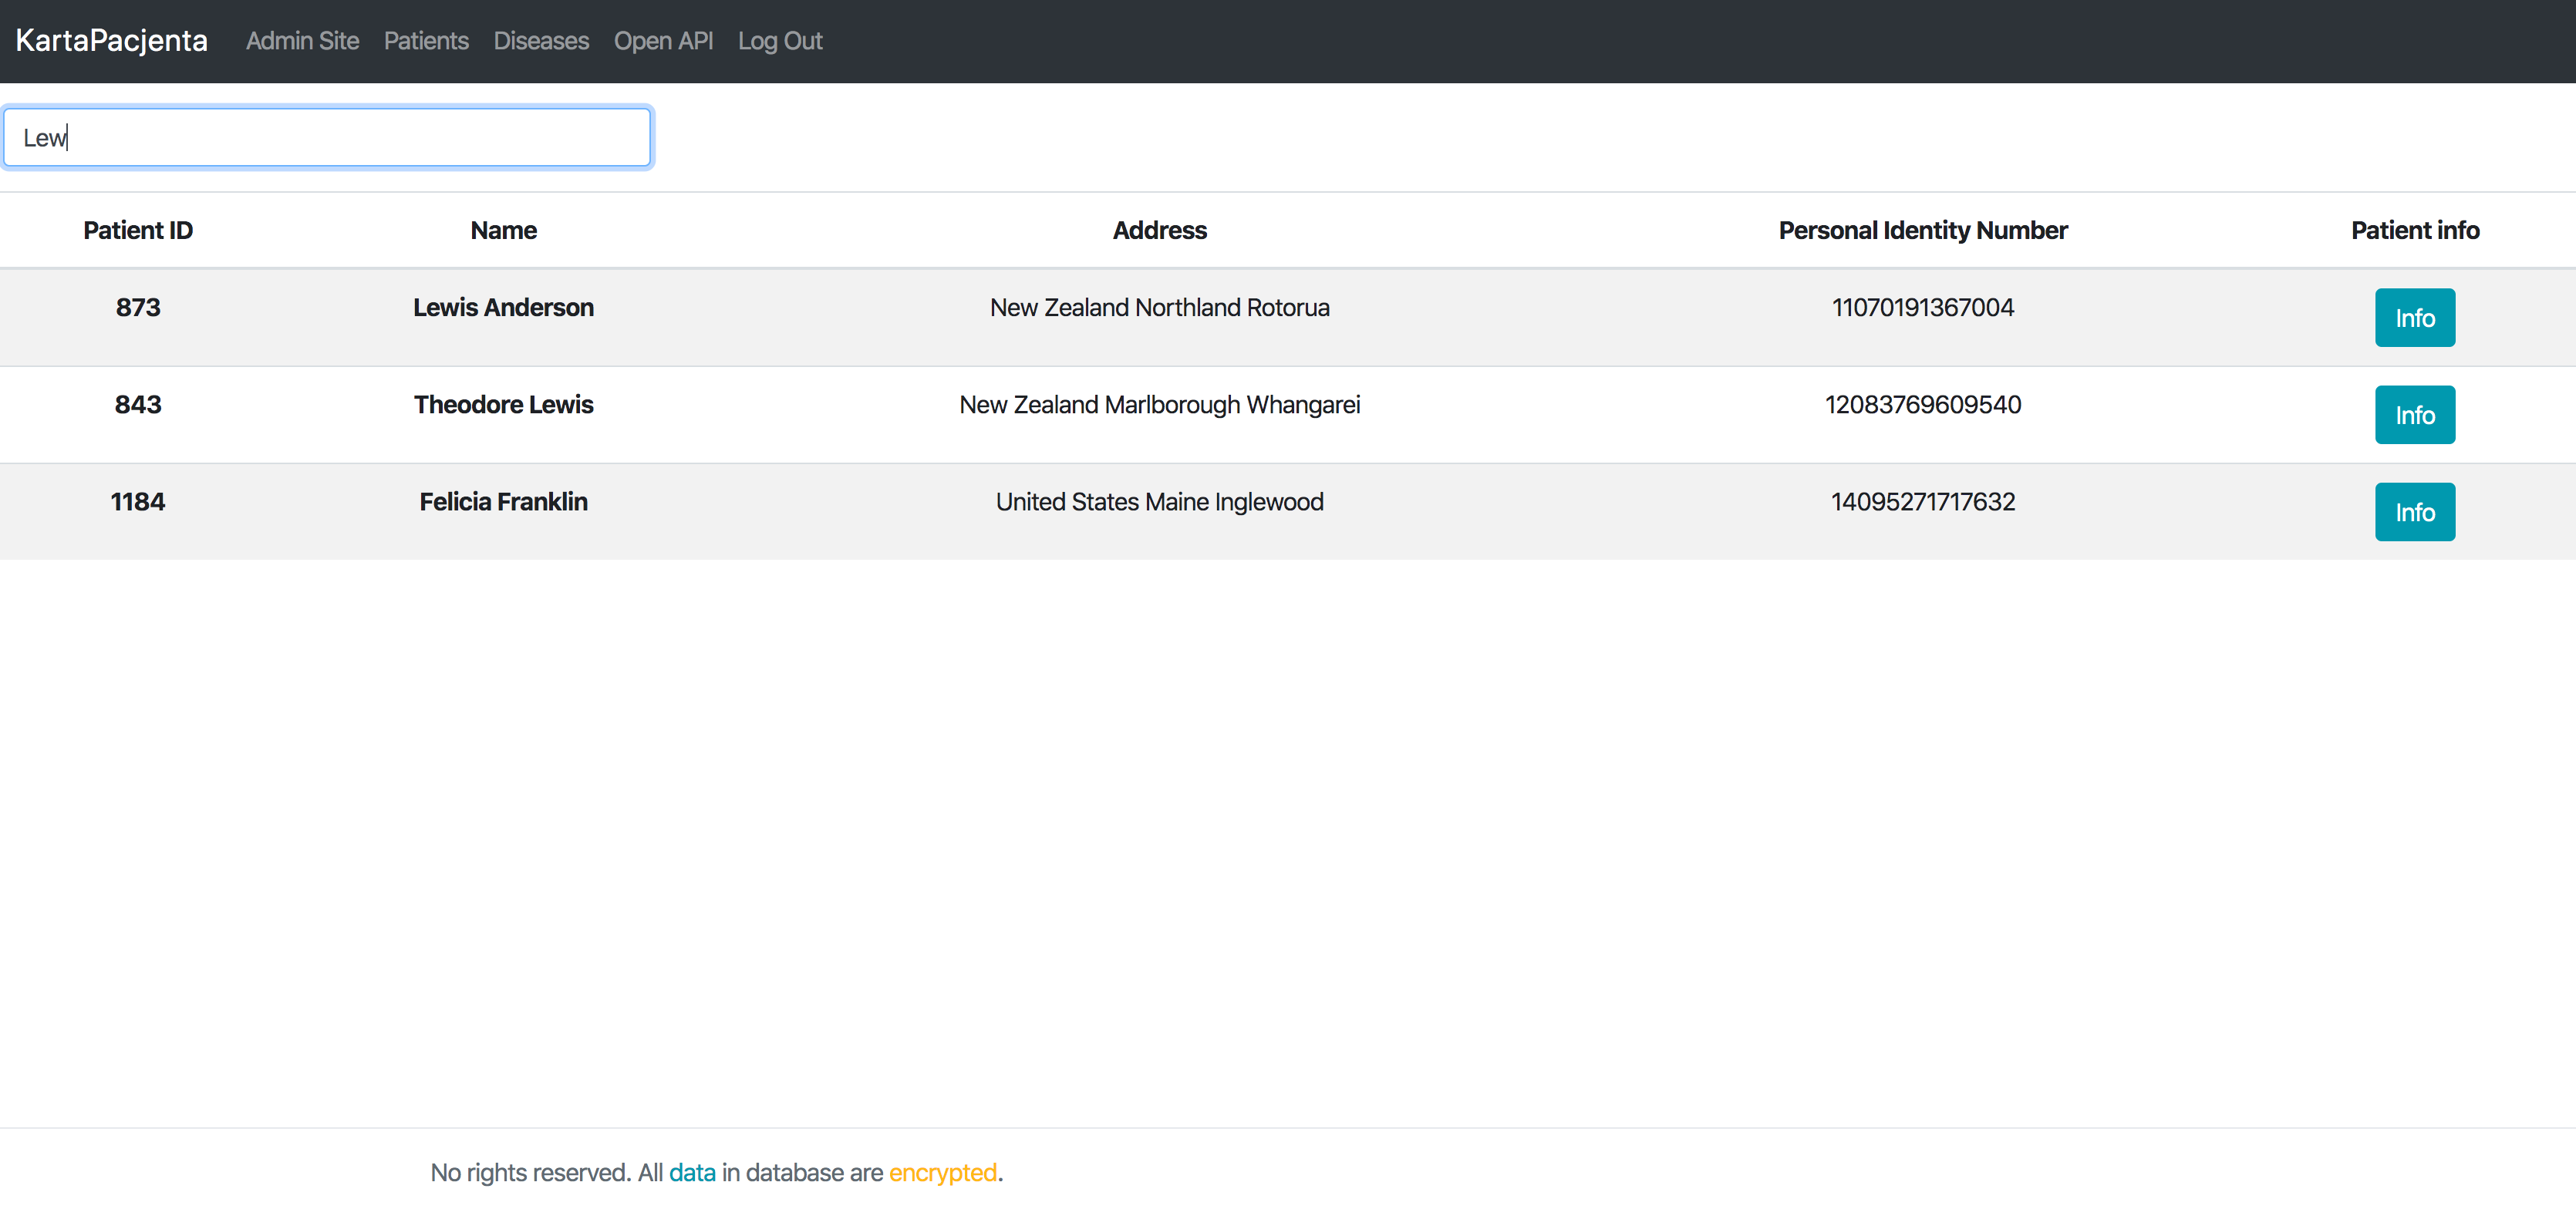
\includegraphics[width=15cm]{pictures/service/03-patients}
\caption{Zakładka ze wszystkimi dostępnymi pacjentami.}
\end{figure}

%patient-ingo
\begin{figure}[H]
\centering
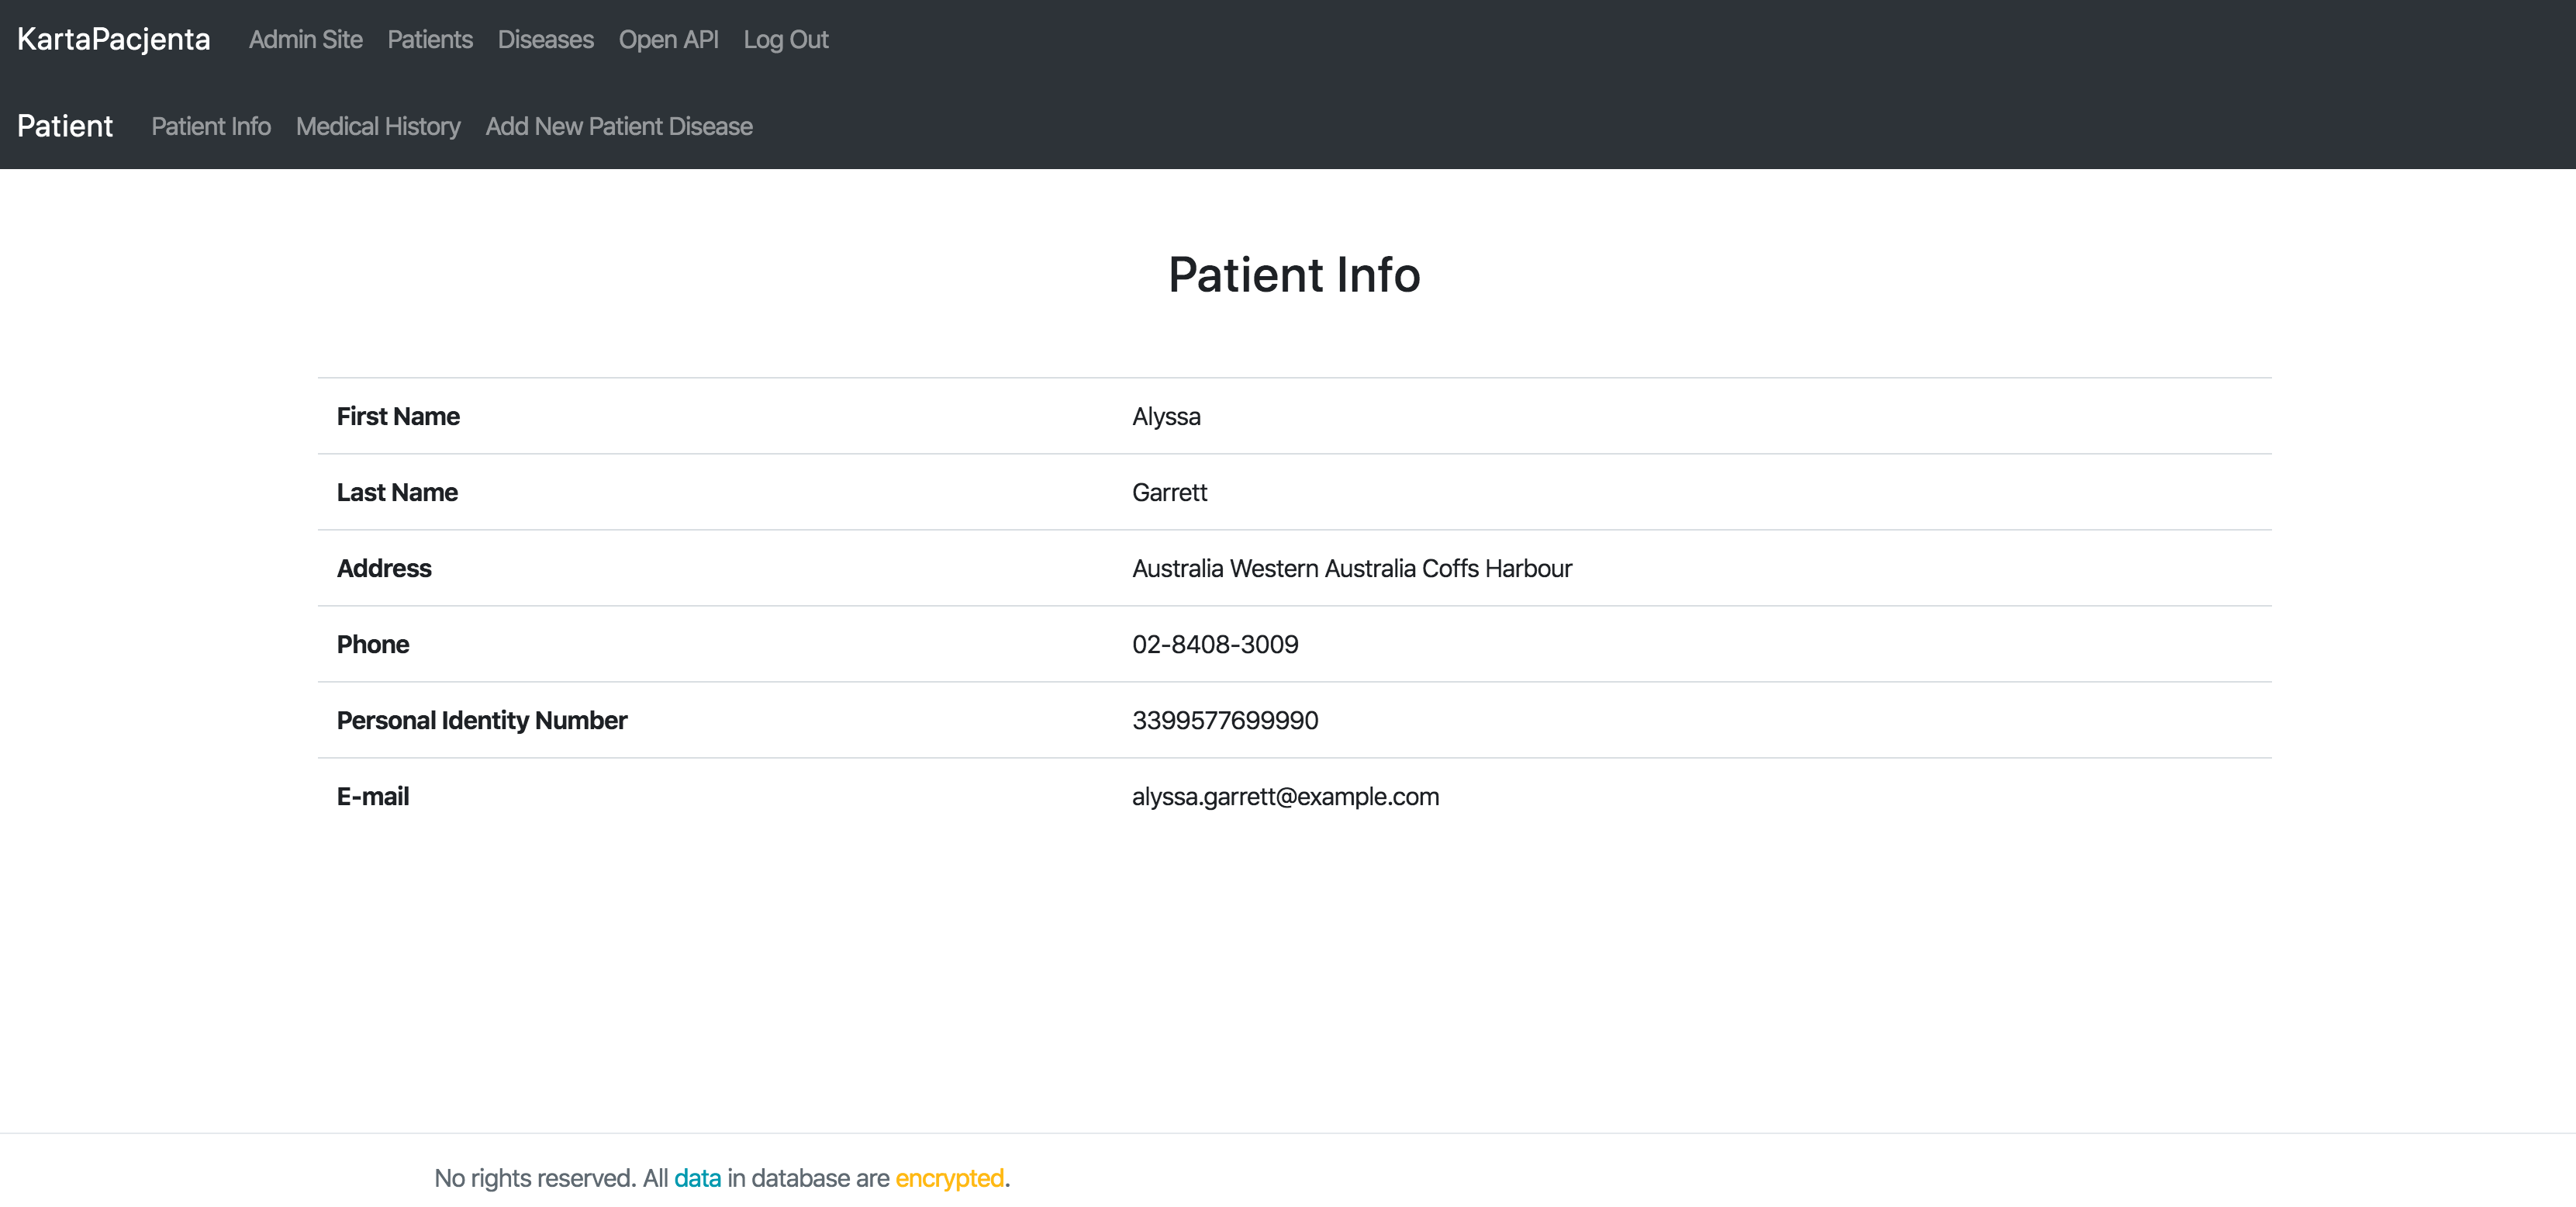
\includegraphics[width=15cm]{pictures/service/05-patient_info}
\caption{Zakładka zawierająca informacje o wybranym pacjencie.}
\end{figure}

% choroby pacjenta
\begin{figure}[H]
\centering
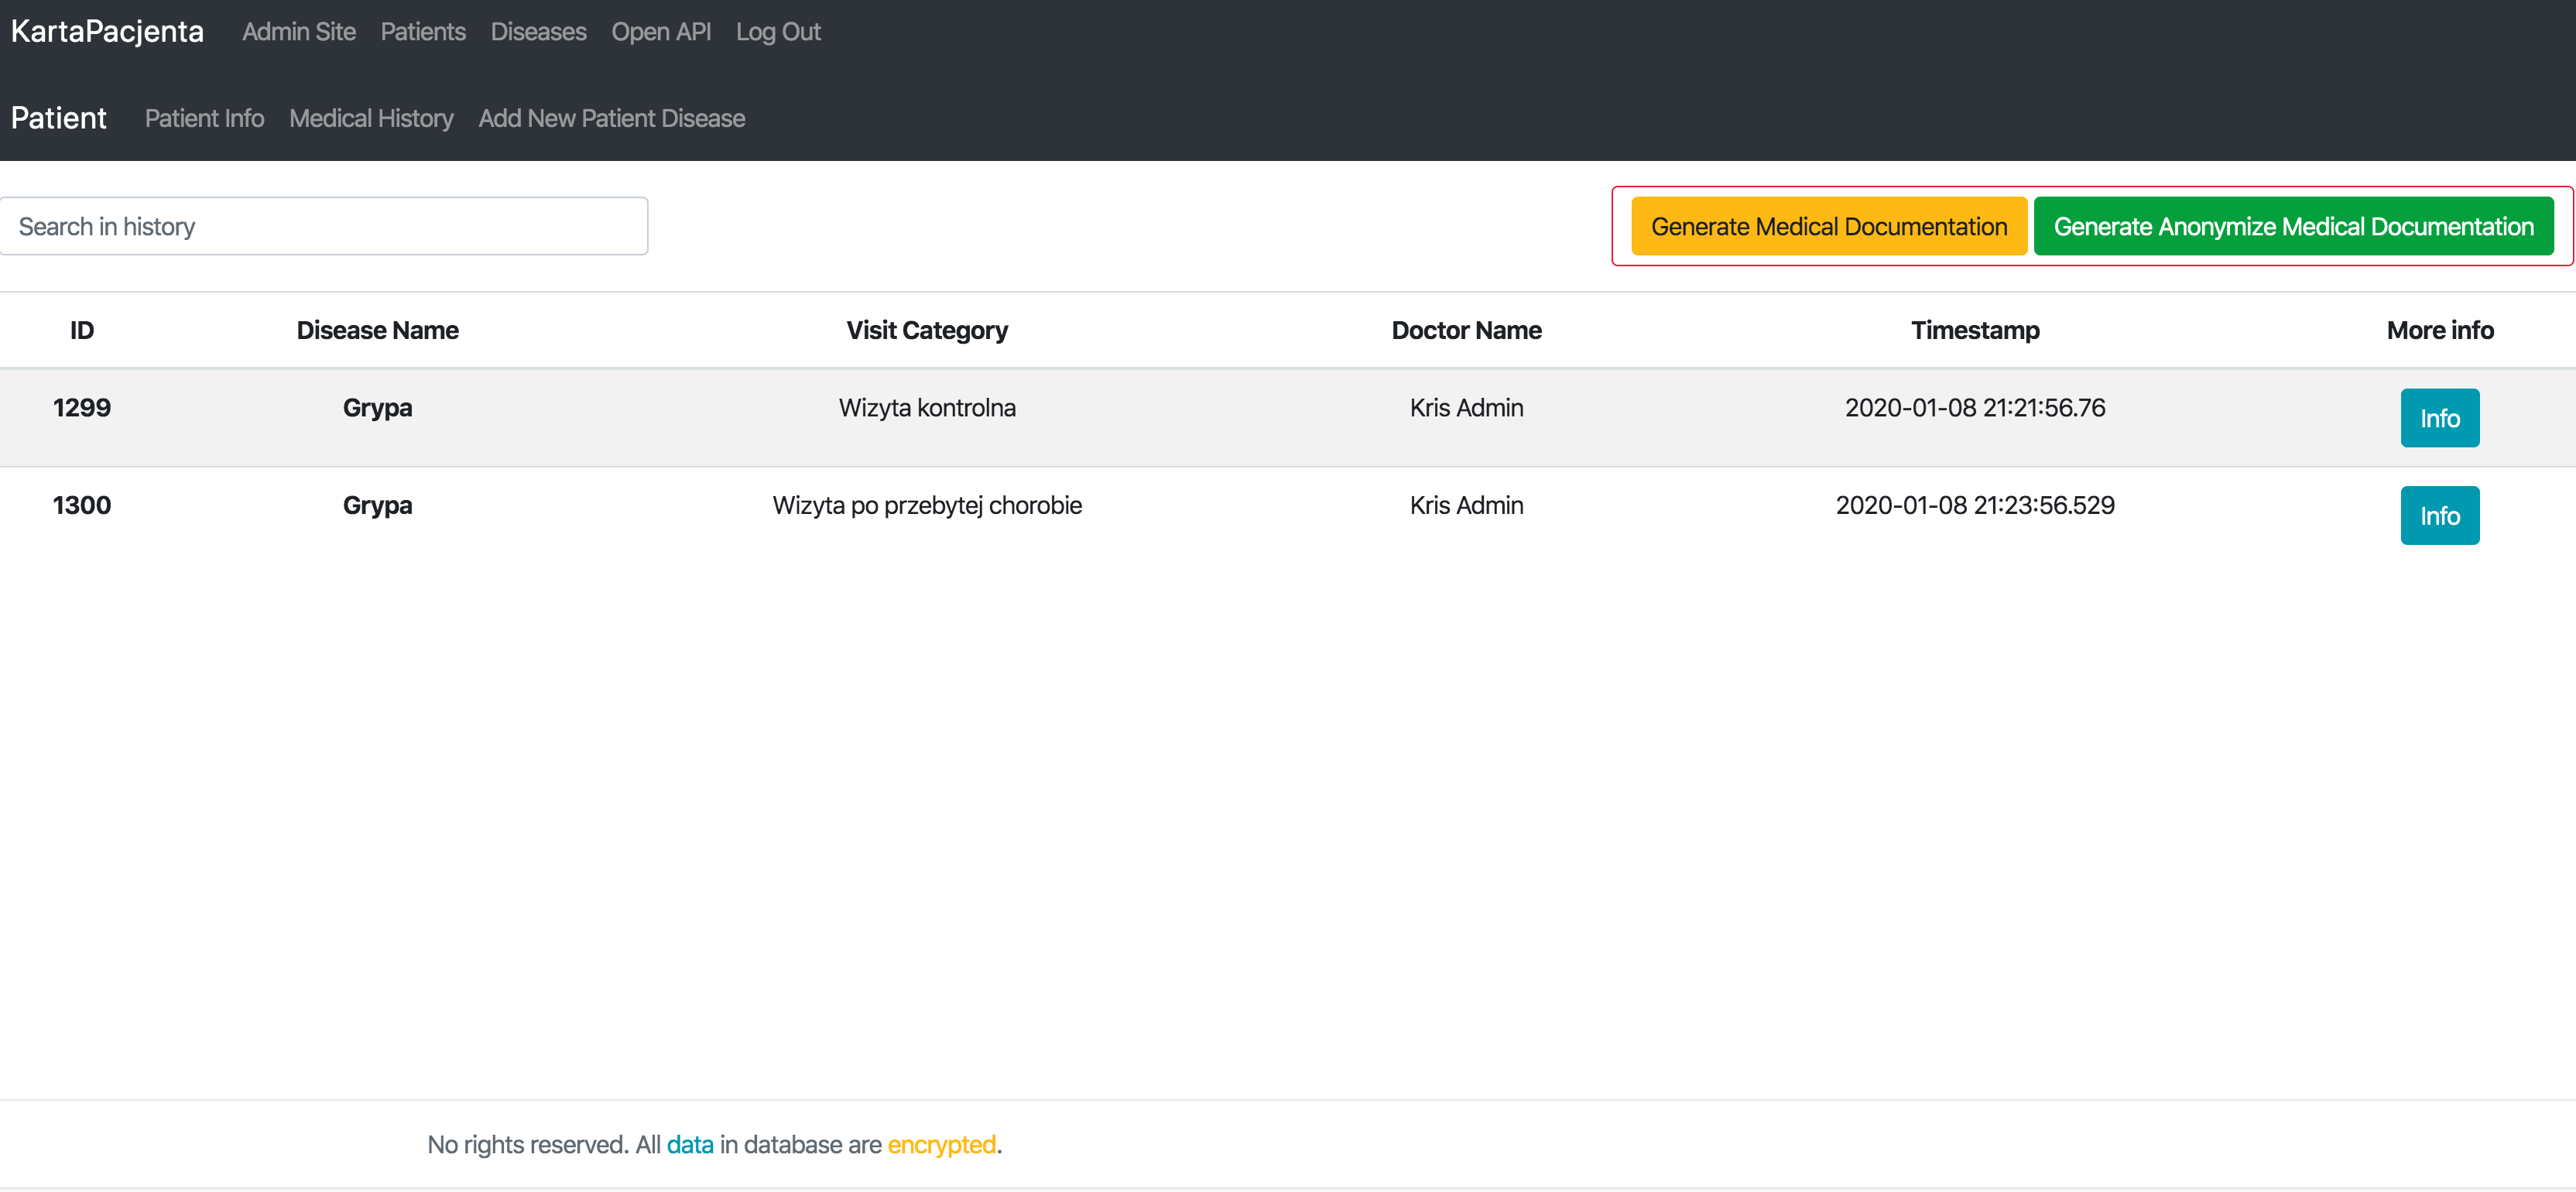
\includegraphics[width=15cm]{pictures/service/06-choroby_pacjenta}
\caption{Historia wizyt pacjenta.}
\end{figure}

% historia normalna
\begin{figure}[H]
\centering
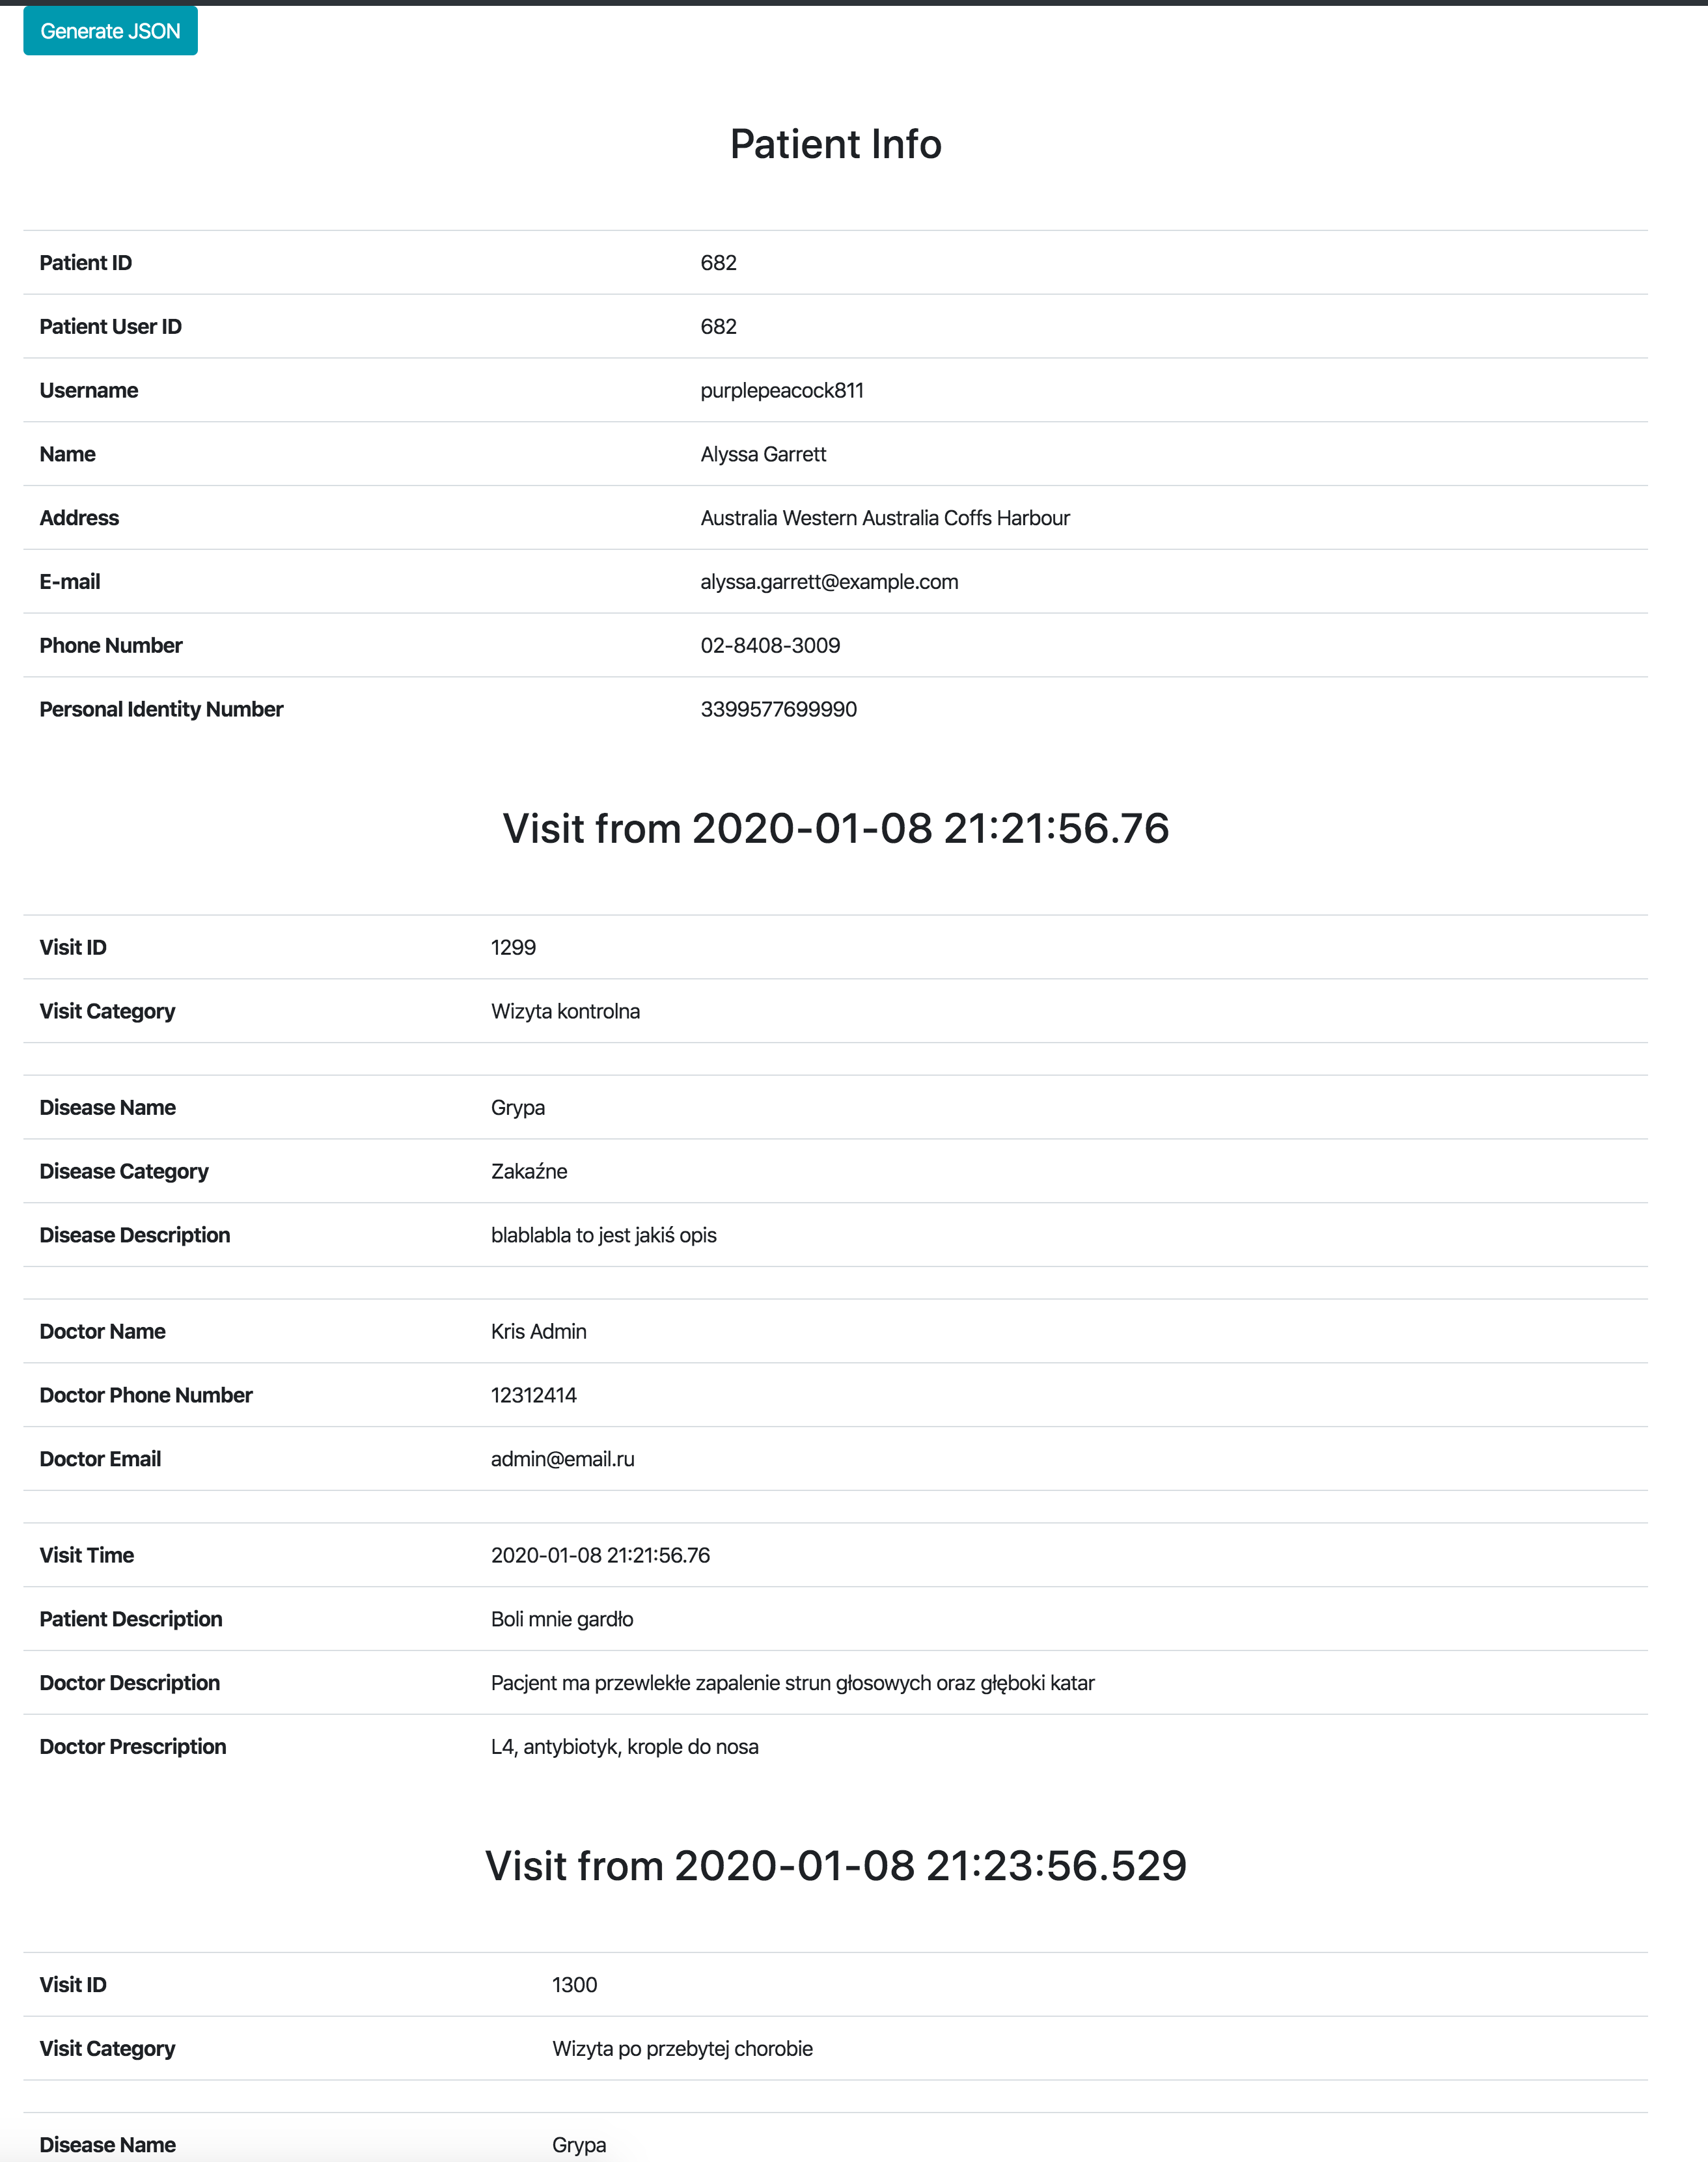
\includegraphics[width=15cm]{pictures/service/09-history_normal}
\caption{Szczegółowa historia wizyt}
\end{figure}

% json normal
Serwis umożliwia wygenerowanie danych o pacjencie i przebytych chorobach w zunifikowanym formacie \textit{JSON}. Jest to możliwe na stronie związanej w historią choroby pacjenta, przedstawionej na rysunku \ref{history_pic}.
\begin{figure}[H]
\centering
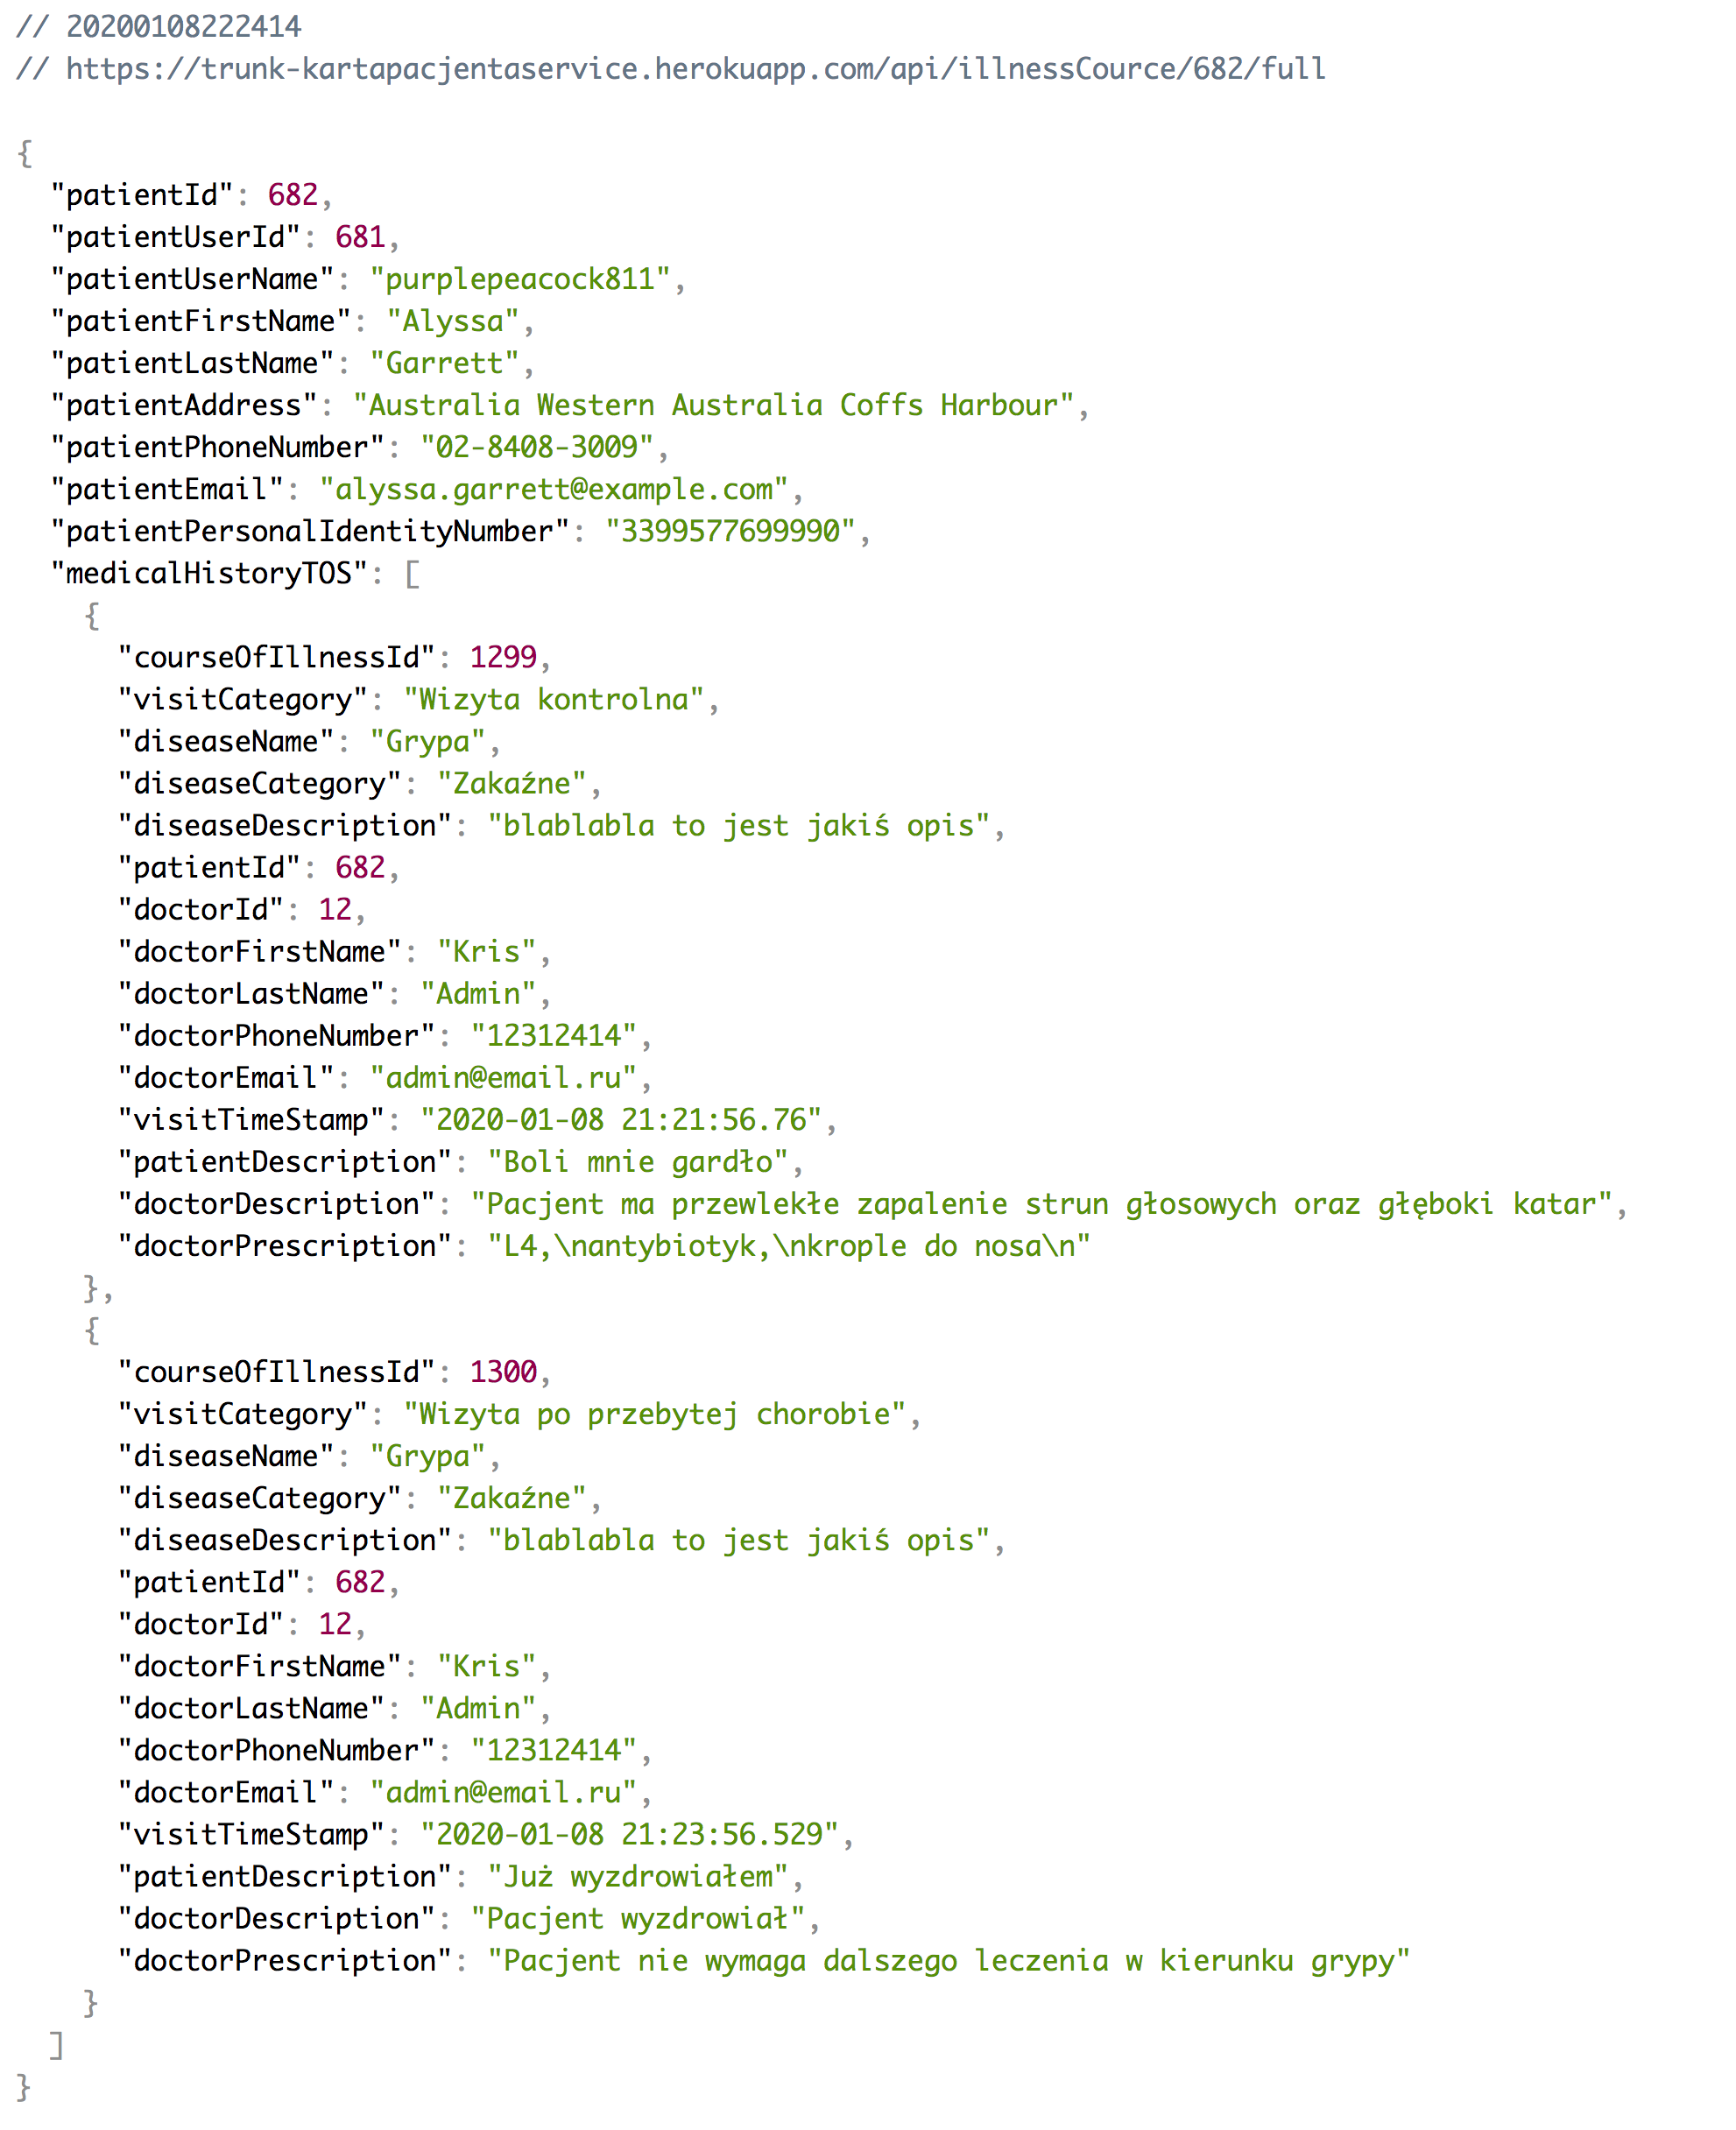
\includegraphics[width=15cm]{pictures/service/07-json_normal}
\caption{Dane pacjenta i jego choroby w formacie JSON.}
\end{figure}

% swagger
Serwis posiada także możliwość przetestowania punktów końcowych (ang. \textit{endpoint}). Funkcjonalność dostępna jest na  \href{https://trunk-kartapacjentaservice.herokuapp.com/swagger-ui.html#/}{stronie}.

\subsection{Testowanie aplikacji}
Do przetestowania wszystkich funkcji aplikacji ,,Karta Pacjenta'' wymagane jest, aby skorzystać z konta administratora - konta różnych użytkowników posiadają różne uprawnienia. Administrator ma dostęp do wszystkich możliwych miejsc na stronie. Podczas testowania aplikacji proszę używać konta:\\
\begin{center}
\label{credentials}
login: admin\\
hasło: admin
\end{center}

\section{Wykorzystane technologie}
\section{Wykorzystane technologie}
\begin{itemize}
	\item Język Programowania \textbf{Java} - (ang. \textit{backend}),
	\item Szkielet aplikacyjny (ang. \textit{framework}) \textbf{Spring Boot} - wykorzystywany do programowania logiki serwisu internetowego (ang. \textit{backend}),
	\item Szkielet aplikacyjny (ang. \textit{framework}) \textbf{Spring Security} - wykorzystywany do zabezpieczenia dostępów do punktów dostępowych serwisu internetowego (ang. \textit{endpoint}),
	\item Szkielet aplikacyjny (ang. \textit{framework}) \textbf{Angular CLI} - wykorzystywany do utworzenia warstwy wizualnej aplikacji (ang. \textit{frontend}),
	\item System zarządzania relacyjnymi bazami danych \textbf{PostgreSQL}.
\end{itemize}


\section{Implementacja}
\section{Implementacja}
\subsection{Kontrola wersji}
Do pracy zespołowej wykorzystano narzędzie \textit{Git}. Umożliwiło ono sprawne dzielenie się zmianami w kodzie, zarządzanie i wersjonowanie zmian.

\subsection{Baza danych}
Na rysunku \ref{diagram} przedstawiony jest diagram ER schematu bazy danych.
\begin{figure}[H]
\centering
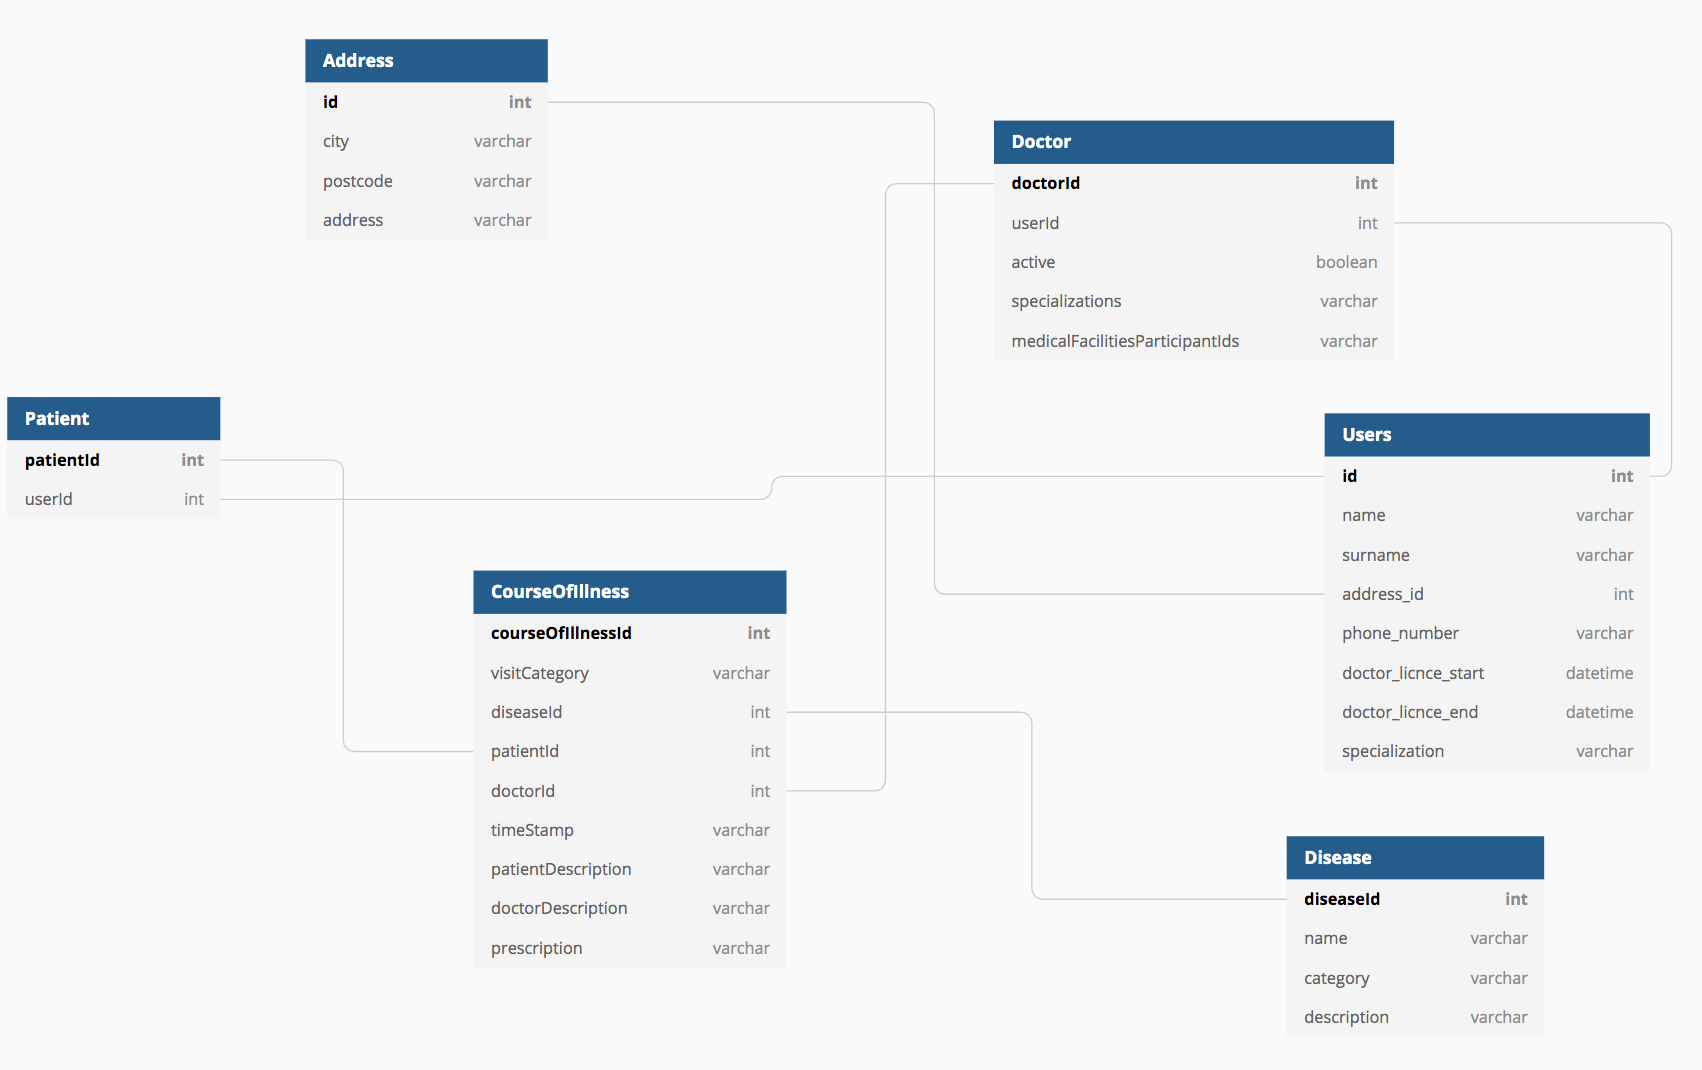
\includegraphics[width=15cm]{pictures/diagram}
\caption{Diagram ER bazy danych}
\label{diagram}
\end{figure}


Poniżej przedstawiono kod SQL wykorzystywany do inicjalizacji bazy danych:
\begin{lstlisting}[
           language=SQL,
           showspaces=false,
           basicstyle=\ttfamily,
           numbers=left,
           numberstyle=\tiny,
           commentstyle=\color{gray}
        ]
CREATE TABLE "Address" (
  "id" SERIAL PRIMARY KEY NOT NULL,
  "city" varchar,
  "postcode" varchar,
  "address" varchar
);

CREATE TABLE "Users" (
  "id" SERIAL PRIMARY KEY NOT NULL,
  "name" varchar,
  "surname" varchar,
  "address_id" int,
  "phone_number" varchar,
  "doctor_licnce_start" datetime,
  "doctor_licnce_end" datetime,
  "specialization" varchar
);

CREATE TABLE "Disease" (
  "diseaseId" SERIAL PRIMARY KEY NOT NULL,
  "name" varchar,
  "category" varchar,
  "description" varchar
);

CREATE TABLE "Doctor" (
  "doctorId" int PRIMARY KEY,
  "userId" int,
  "active" boolean,
  "specializations" varchar,
  "medicalFacilitiesParticipantIds" varchar
);

CREATE TABLE "Patient" (
  "patientId" int PRIMARY KEY,
  "userId" int
);

CREATE TABLE "CourseOfIllness" (
  "courseOfIllnessId" int PRIMARY KEY,
  "visitCategory" varchar,
  "diseaseId" int,
  "patientId" int,
  "doctorId" int,
  "timeStamp" varchar,
  "patientDescription" varchar,
  "doctorDescription" varchar,
  "prescription" varchar
);

ALTER TABLE "Users" 
ADD FOREIGN KEY ("address_id") 
REFERENCES "Address" ("id");

ALTER TABLE "Doctor" 
ADD FOREIGN KEY ("userId") 
REFERENCES "Users" ("id");

ALTER TABLE "Patient" 
ADD FOREIGN KEY ("userId") 
REFERENCES "Users" ("id");

ALTER TABLE "CourseOfIllness" 
ADD FOREIGN KEY ("diseaseId") 
REFERENCES "Disease" ("diseaseId");

ALTER TABLE "CourseOfIllness" 
ADD FOREIGN KEY ("patientId") 
REFERENCES "Patient" ("patientId");

ALTER TABLE "CourseOfIllness" 
ADD FOREIGN KEY ("doctorId") 
REFERENCES "Doctor" ("doctorId");
\end{lstlisting}


\subsection{Logika aplikacji (ang. \textit{backend})}

\subsubsection{Punkty dostępowe (ang. \textit{enpoint})}
Dzięki ogromnej popularności aplikacji internetowych opartych na języku \textit{Java} oraz \textit{framework'a Spring} możliwe było szybkie wygenerowanie dokumentacji \textit{Open API}. Pod \href{https://trunk-kartapacjentaservice.herokuapp.com/swagger-ui.html} {linkiem} dostępny jest spis wszystkich dostępnych w serwisie endpointów. Wejście w ten link będzie wymagało podania loginu i hasła (dostępnego tutaj: \ref{credentials}).

\subsubsection{Dlaczego REST?}
Zalety REST API:
\begin{itemize}
    \item Bezstanowość klienta - serwer nie ma potrzeby zapamiętywania wcześniejszego stanu, ponieważ zapytania HTTP zawierają wszystkie potrzebne informacje,
    \item Łatwość manipulowania obiektami z poziomu URL - metodami HTTP,
    \item Czytelność wykonywanych działań ze względu na używanie metod HTTP zgodnych z ich przeznaczeniem (np, DELETE do usunięcia danych, GET do pobrania),
    \item Uniwersalność odpowiedzi serwisu - możliwe jest użycie tych samych danych wygenerowanych przez serwis do obsługi aplikacji klienckich na różnych urządzeniach (np. przeglądarka i aplikacja mobilna).
\end{itemize}

\subsubsection{Zabezpieczenie danych - API}
Większość punktów dostępowych dostępnych w serwisie zabezpieczone jest przy użyciu metody \textit{Basic Auth}. Bez podania loginu i hasła niemożliwy jest dostęp do serwisu. Jedyne dostępne bez konieczności autoryzacji punkty dostępowe to te dotyczące logowania i rejestracji.

\subsubsection{Zabezpieczenie danych - baza danych}
Do zabezpieczenia danych skorzystaliśmy z symetrycznego szyfrowania. Informacje przechowywane w bazie są niemożliwe do odszyfrowania bez użycia klucza. Dane w punktach dostępowych są odszyfrowane. Odszyfrowywaniem zajmuje się aplikacja odpowiadająca za logikę serwisu.

\begin{figure}[H]
\centering
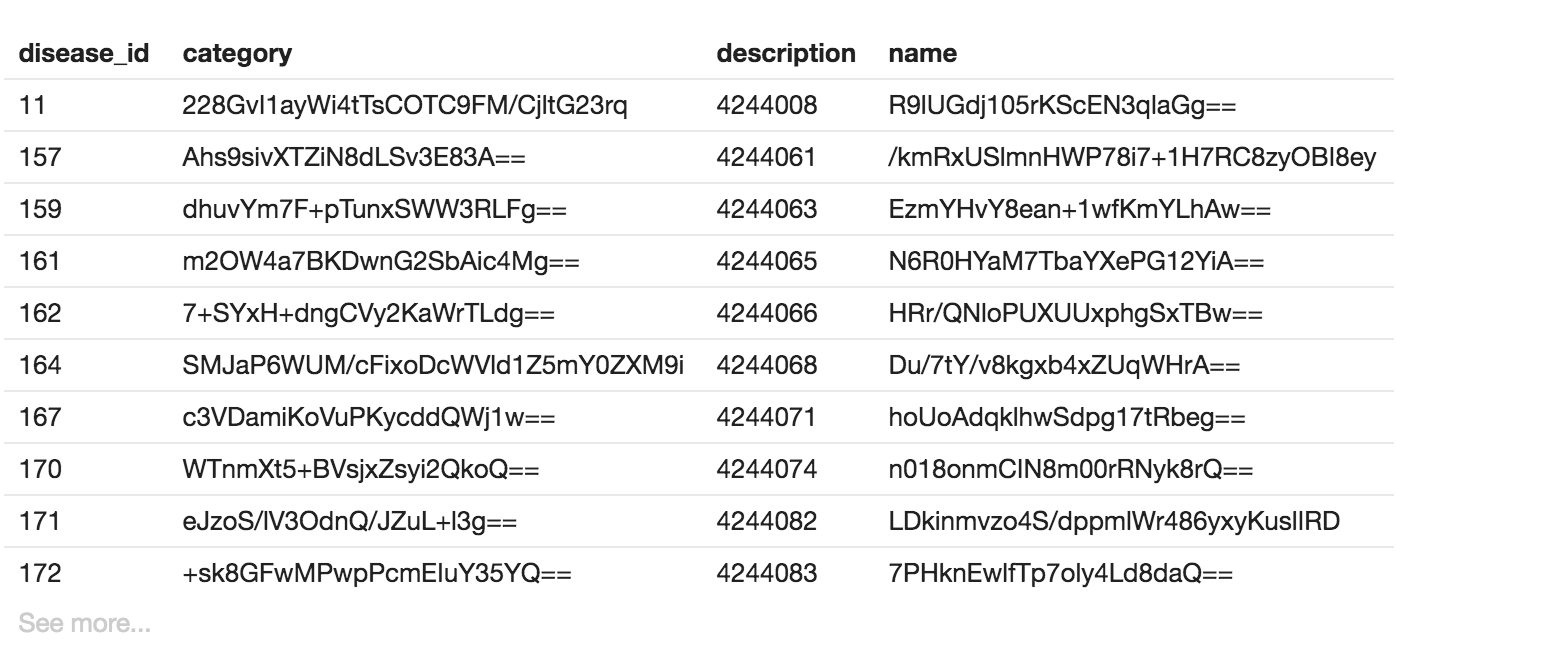
\includegraphics[width=15cm]{pictures/bd-encr}
\caption{Zaszyfrowane krotki bazy danych. Widoczne jest, że ciągi znaków zapisane w bazie danych nie są możliwe do odszyfrowania bez dekodowania.}
\end{figure}

\subsubsection{Ograniczenia}
W trakcie implementacji kolejnych funkcjonalności musieliśmy zmierzyć się z ograniczeniami serwera Heroku. Obsługa zapytań (ang. \textit{request}) jest wykonywana na ograniczonym serwerze, stąd można zaobserwować wydłużony czas oczekiwania na duże zapytanie. Skorzystanie z darmowej domeny sprawia, że funkcjonowanie strony jest po prostu wolne.

\subsubsection{Przyspieszenie}
W trakcie pierwszej wersji implementacji zastosowano wbudowany we framework Spring sterownik będący mostkiem pomiędzy obiektami programu a bazą danych. Jego zastosowanie umożliwiło stosowanie zapytań do bazy przy użyciu specjalnie spreparowanych nazw metod. Wykorzystując ten sposób i np. metodę

\begin{lstlisting}
Optional<Patient> findByUserId(Long userId);
\end{lstlisting}

automatycznie generuje się kod SQL, który odpowiada za znalezienie użytkownika o zadanym ID.

Jest to bardzo wygodne, jednak korzystając z możliwości zbudowania własnego zapytania przy użyciu języka SQL udało się uzyskać \textbf{czterokrotne} przyspieszenie związane ze stosowaniem bardziej złożonych zapytań. Wstrzyknięcie zapytania SQL zaimplementowane jest w następujący sposób:

\begin{lstlisting}
@Query(
value = "select distinct patients.patient_id, 
	my_app_users.* from my_app_users " +
	"join patients\n" +
	"on my_app_users.user_id=patients.user_id",
	nativeQuery = true)
List<PatientInfoTO> findAllPatients();
\end{lstlisting}



\subsubsection{Możliwości dotyczące rozwoju - przyspieszenie}
Przyspieszenie może zostać uzyskane np. poprzez zastosowanie architektury mikro-serwisowej, tak by każda atomowa operacja mogła zostać wykonywana niezależnie. Zapewniłoby to dużą skalowalność systemU i pod dużym obciążeniem przełożyłoby się to na przyspieszenie. 



\subsection{Aplikacja - frontend}
\subsubsection{Działanie warstwy wizualnej}
\subsubsection{Prostota implementacji i wieloplatformowość}
\subsubsection{Rola warstwy wizualnej aplikcji}


\subsection{Testy obciążeniowe}
\subsubsection{Testowane zagadnienia}
\subsubsection{Wielowątkowość}
\subsubsection{Szybkość działania aplikacji}
\subsubsection{Rola testów w rozwoju aplikacji}



\nocite{craigspring}
\nocite{sql}
\nocite{algorytmy}
\nocite{springporadnik}
\nocite{springsecurity}
\nocite{rest}
\nocite{angular}

\bibliographystyle{unsrtnat}
\bibliography{references}

\end{document}

% PUNKTORY
% \begin{itemize}
% \item Public Documents
% \item All Documents
% \item Create Document
% \end{itemize}

% obrazek
% \begin{figure}[H]
% \centering
% \includegraphics[width=15cm]{pictures/deszyf_mycbc.png}
% \caption{Wykres zależności czasu deszyfrowania [ms] od wielkości pliku [MB] z uwzględnieniem własnej implementacji szyfru CBC}
% \label{pictures/szyfrowanie.png}
% \end{figure}